\documentclass[12pt, oneside]{article}
 
\usepackage{graphicx}
\usepackage{hyperref}
\graphicspath{ {Images/} }

\begin{document}
\thispagestyle{empty}
\begin{center}
\begin{minipage}{0.75\linewidth}
    \centering

    {\uppercase{\Large COS 301 Assignment\par}}
   	{\uppercase{\Large Group 5 B \par}}
    \vspace{1cm}
    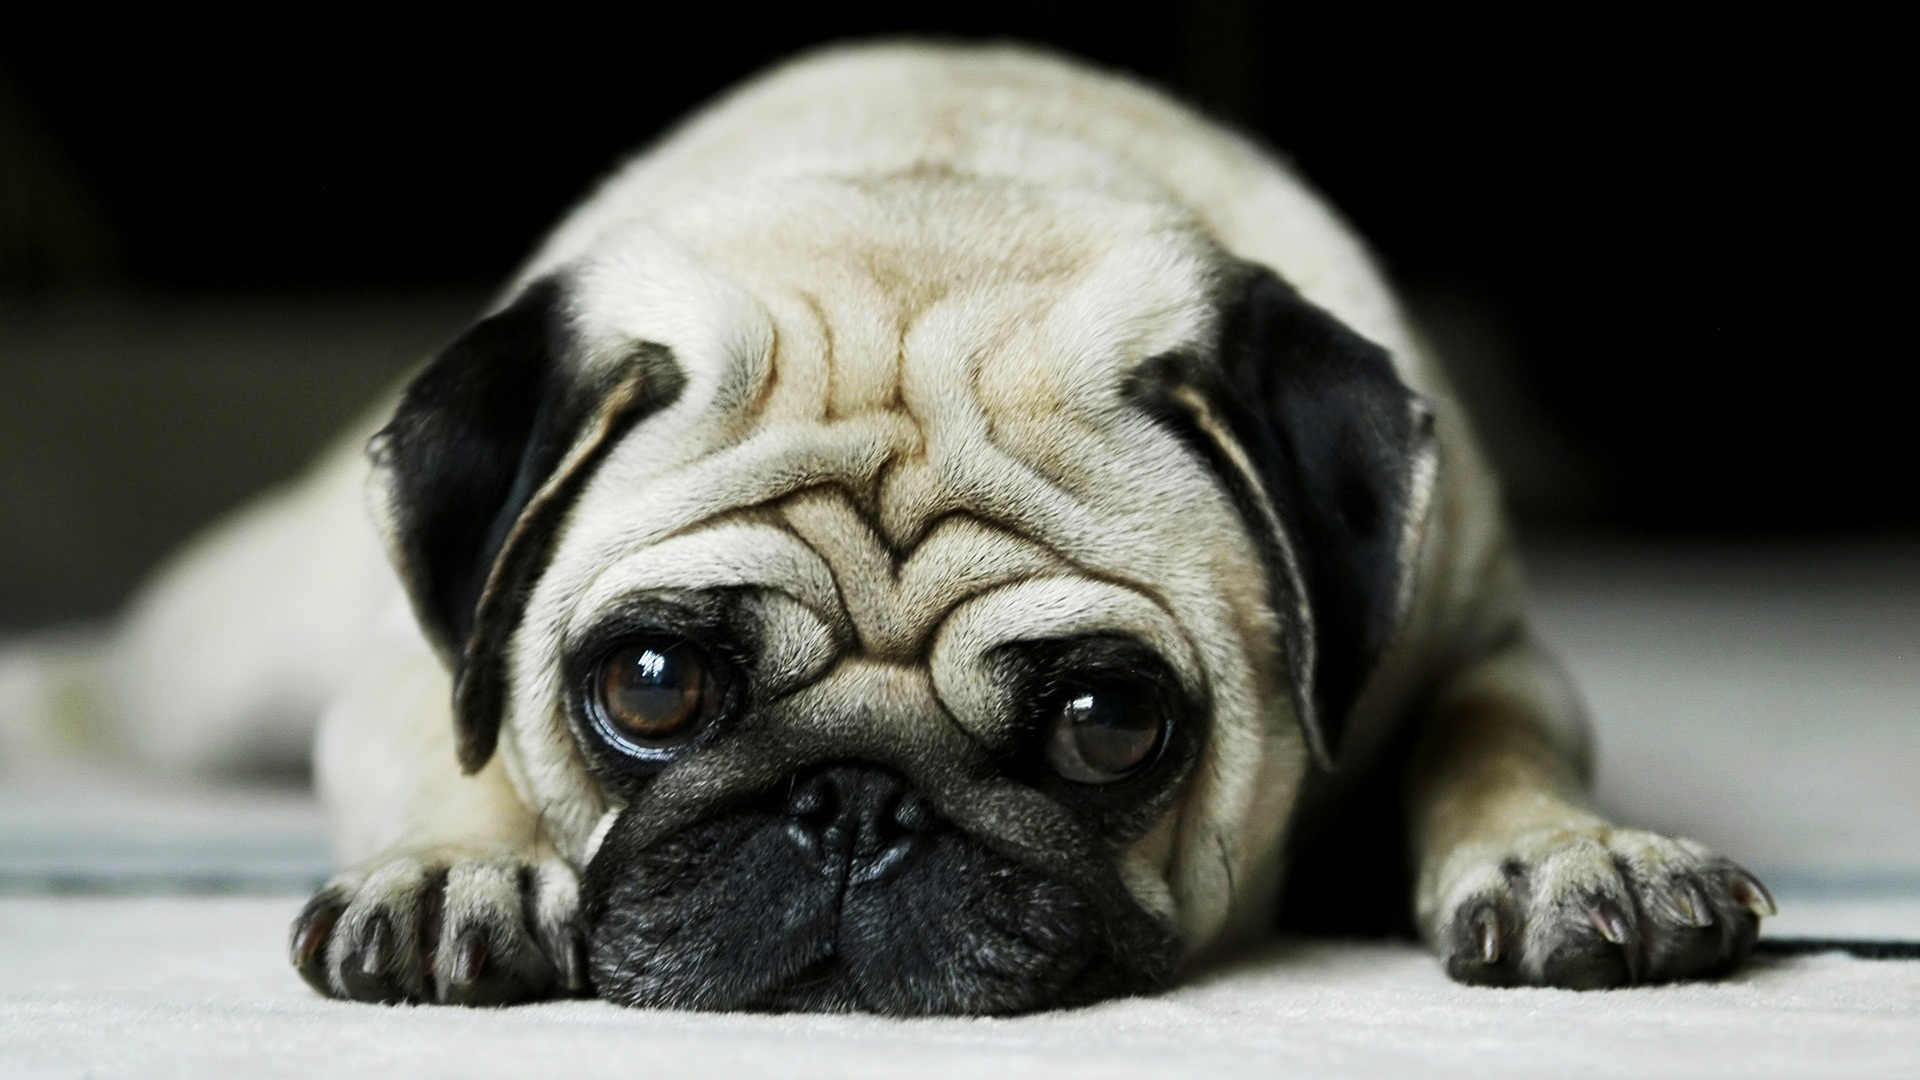
\includegraphics[scale=0.3]{example} %Example is the name of the image

    {\normalsize Sebastian Gerber (12213749)\par}
    {\normalsize Godfrey Mathe (13103394)\par}
    {\normalsize Shaun Meintjes (13310896)\par}
    {\normalsize Duran Cole (13329414)\par}
    {\normalsize Isabel Nel (1307030)\par}
    \vspace{1cm}
    
    {\Large February 2015}
\end{minipage}
\end{center}
\clearpage

\newpage

\section{Introduction}
The idea behind the 'Buzz' project is to find ways to enhance teaching and improve the learning of students through the use of online discussions.  The 'Buzz' will be an online forum where students can express their views on specific work topics, thus students will be able to see the work from other students perspective's and be able to discuss problems and find solutions creating an educational environment while allowing for social interactivity among students.

The idea is to create a fun, rewarding and educational environment, thus students will be rewarded for participating in this online forum by being 'leveled up' according to contributions on the forum. When a student reaches a new level he/she will have more privileges such as being able to start their own thread and having access to more functionality. All users will also be able to see each other's levels - in this way we try to motivate students to 'level up' to also receive those privileges.   

By having students communicating about work related to subjects the lecturers will also be able to view the discussions and thus see what problems and questions students have about the work and can address these again in class if needed. Lecturers on the other hand will also have a lot more privileges than students and can at any time start a new thread and discussions and so forth. 

The forum needs to be user-friendly to help inexperienced users to easily navigate and find their way around the forum thus it also needs to be well and logically organized. It should also raise excitement in students to want to participate in discussions or just go onto the forum and read about work covered during lectures to get a better understanding. 

	
\section{Functional requirements and application design}
	\subsection{Use case prioritization}
		\subsubsection{Critical}
			\begin{itemize}
				\item Login
				\item Logout
				\item Post
				\item Thread
				\item Buzz Space
				\item User Management(Profile)
			 \end{itemize}
		\subsubsection{Important}
			\begin{itemize}
				\item Search
				\item Voting
				\item Notifications
			 \end{itemize}
		\subsubsection{Nice to Have}
			\begin{itemize}
				\item Request
			 \end{itemize}
	\subsection{Use case/Services contracts}
			\subsubsection{Login}
				Pre-Conditions : \begin{itemize}
							\item Must not be logged in.
						     \end{itemize}
				Post-Conditions : \begin{itemize}
							\item If login succesful, user will be logged in.
							\item If login failed. user will be asked to resubmit
						     \end{itemize}
			\subsubsection{Logout}
				Pre-Conditions : \begin{itemize}
							\item Must be logged in.
						     \end{itemize}
				Post-Conditions : \begin{itemize}
							\item User is logged out.
						     \end{itemize}
			\subsubsection{Post}
				Pre-Conditions : \begin{itemize}
							\item Must be logged in.
							\item A thread should exist.
						     \end{itemize}
				Post-Conditions : \begin{itemize}
							\item Post is created.
						     \end{itemize}
			\subsubsection{Buzz Space}
				Pre-Conditions : \begin{itemize}
							\item To create a Buzz Space, user must be logged in and user must be authorized.
							\item To delete a Buzz Space the Buzz Space must exist and user must own the Buzz Space.
							\item To edit a Buzz Space, the Buzz Space must exist and user must own Buzz Space.
						     \end{itemize}
				Post-Conditions : \begin{itemize}
							\item Buzz Space is either created, deleted or edited according to the functionality used.
						     \end{itemize}
			\subsubsection{Request}
				Pre-Conditions : \begin{itemize}
							\item Must be logged in.
						     \end{itemize}
				Post-Conditions : \begin{itemize}
							\item Request is sent.
						     \end{itemize}
			\subsubsection{Thread}
				Pre-Conditions : \begin{itemize}
							\item Only Authorised persons may use this functionality.
							\item Buzz Space needs to exist .
							\ No such thread sould already exist.
						     \end{itemize}
				Post-Conditions : \begin{itemize}
							\item A new Thread now exists under which people can create posts.
						     \end{itemize}
			\subsubsection{Voting}
				Pre-Conditions : \begin{itemize}
							\item Must not be logged in.
							\item User has not yet voted.
						     \end{itemize}
				Post-Conditions : \begin{itemize}
							\item User voted.
						     \end{itemize}
			\subsubsection{Search}
				Pre-Conditions : \begin{itemize}
							\item User needs to enter a search request.
						     \end{itemize}
				Post-Conditions : \begin{itemize}
							\item Search results are returned.
						     \end{itemize}	
			\subsubsection{Notifications}
				Pre-Conditions : \begin{itemize}
							\item Must not be logged in to see notifications.
						     \end{itemize}
				Post-Conditions : \begin{itemize}
							\item Notification is displayed to user.
						     \end{itemize}

	\subsection{Required functionality}
	\begin{center}

			 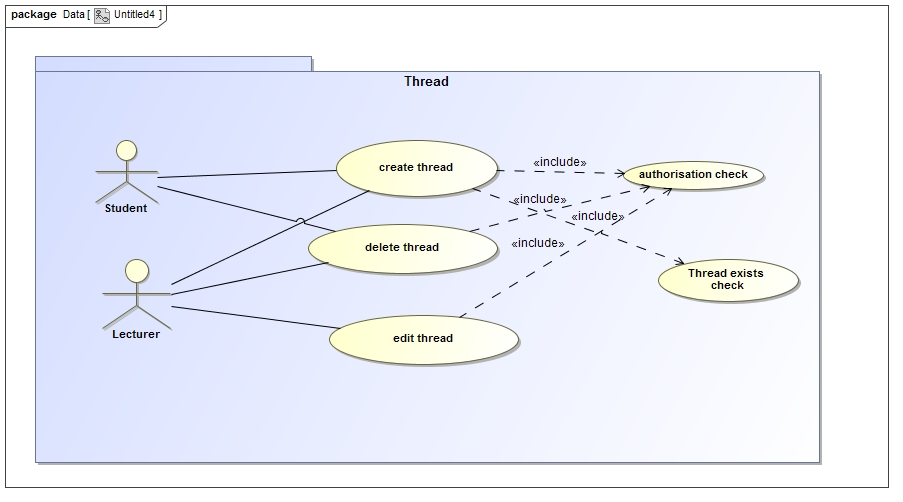
\includegraphics[scale=0.5]{thread}
			 
			 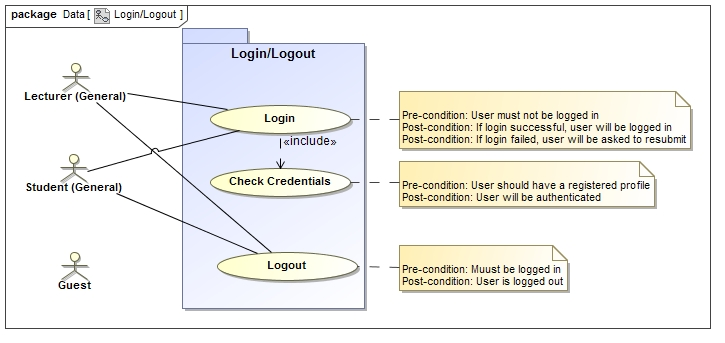
\includegraphics[scale=0.6]{Login_Logout} 
			 
			 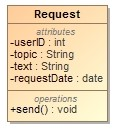
\includegraphics[scale=0.6]{Request}

			 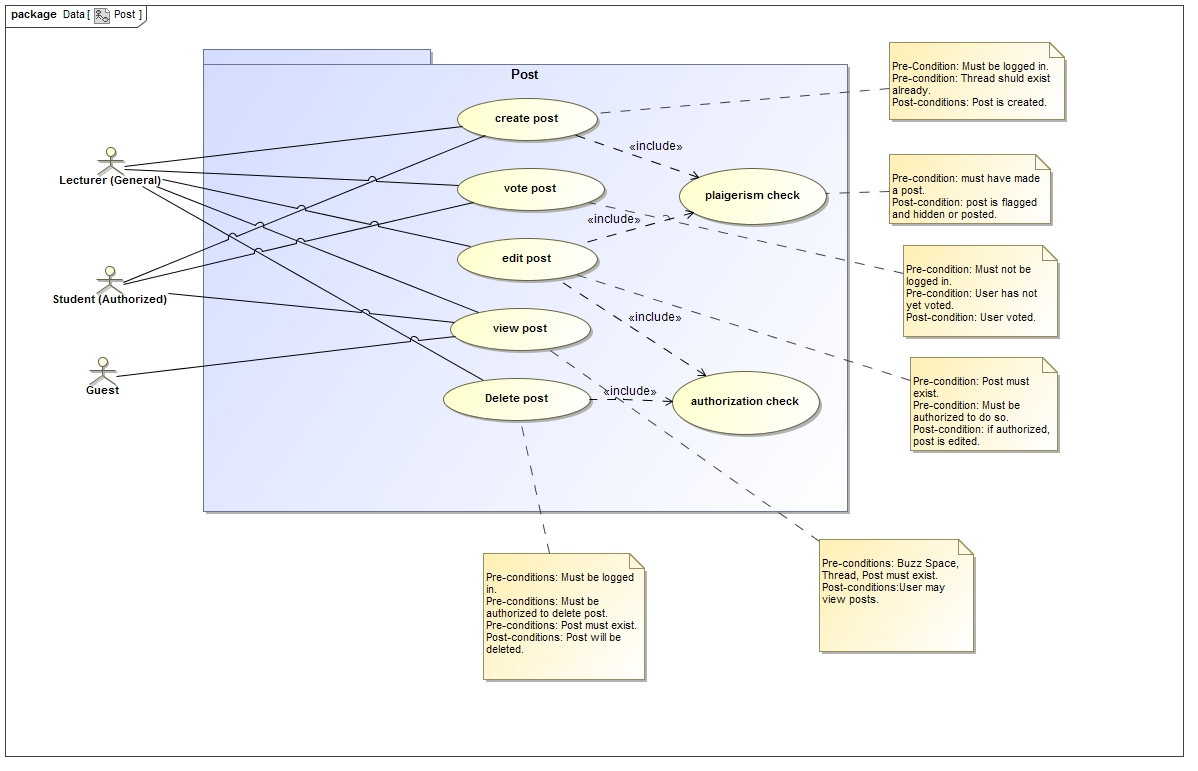
\includegraphics[scale=0.5]{Post} 
			 
			 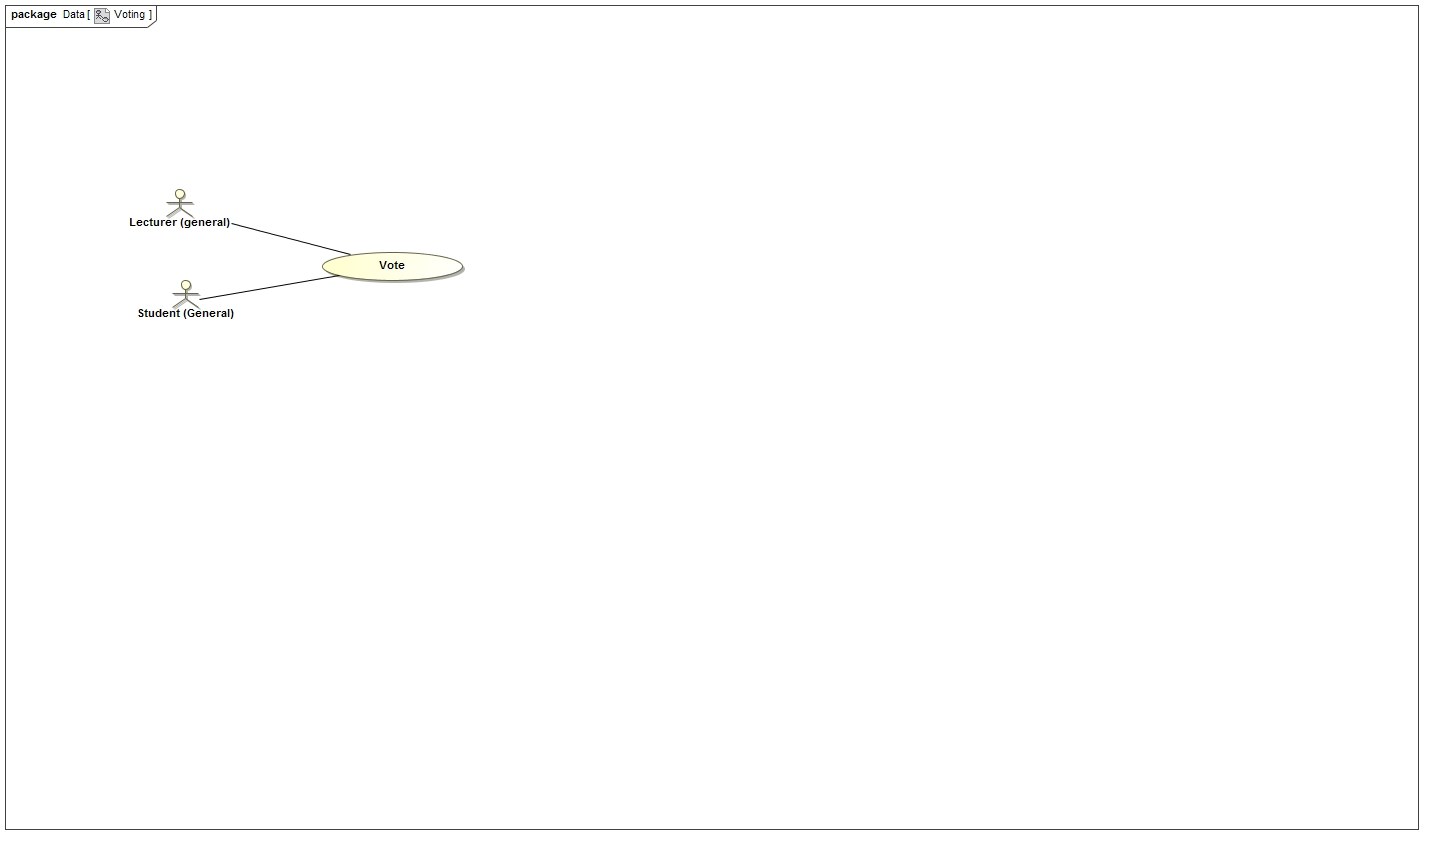
\includegraphics[scale=0.8]{Voting}
			 
			 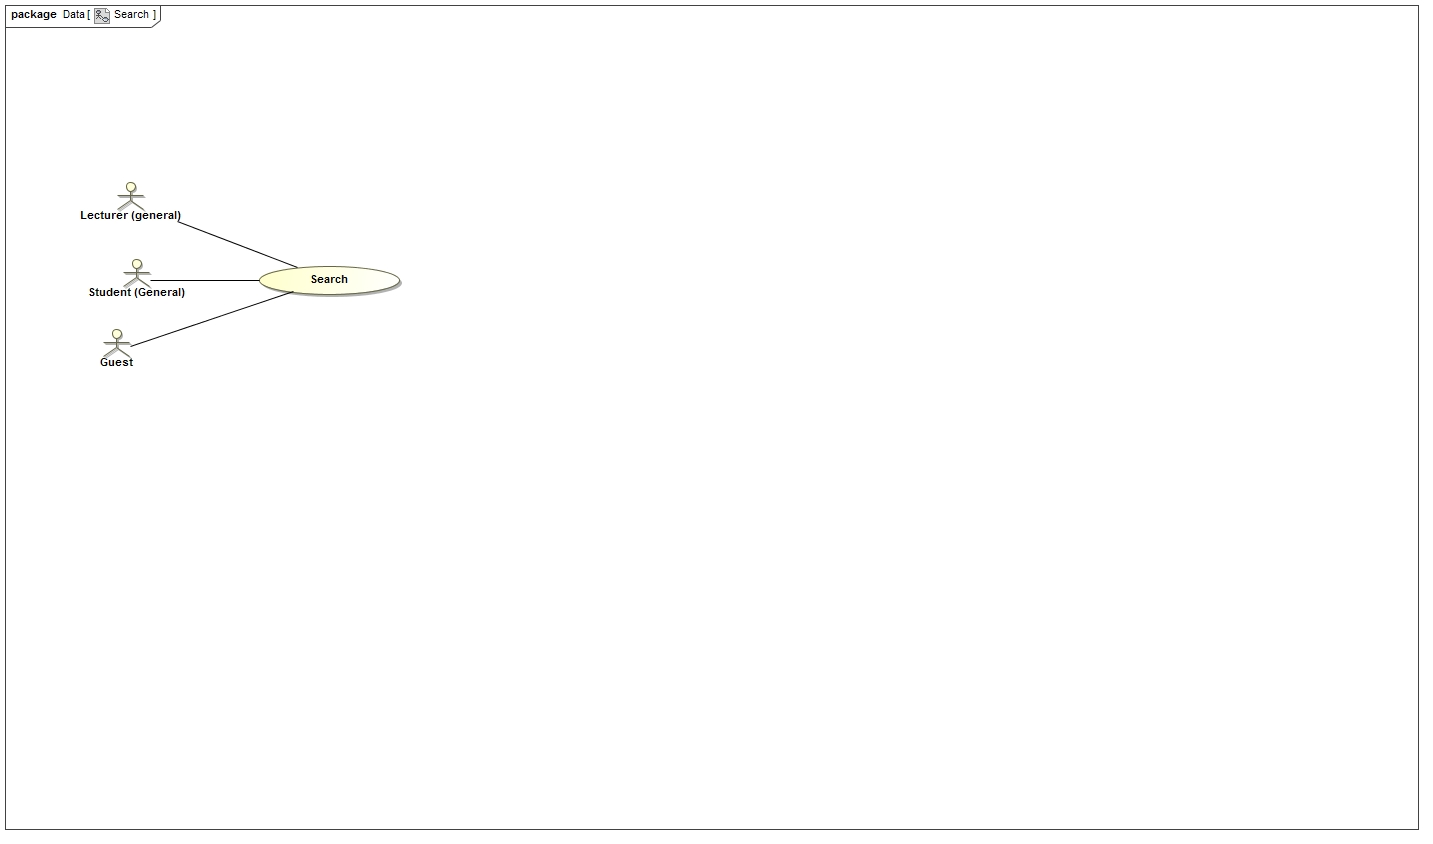
\includegraphics[scale=0.8]{Search}
			 
			 \includegraphics[scale=0.55]{"Buzz Spaces"}
			 
			 
	\end{center}
	\newpage		 
	\subsection{Process specifications}
		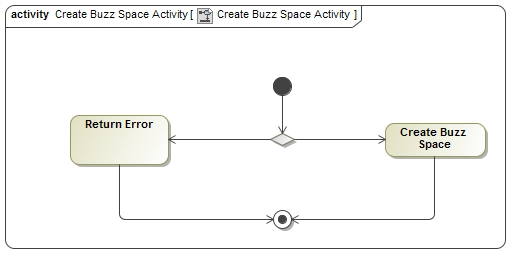
\includegraphics[scale=0.55]{Activity_Diagram__Create_Buzz_Space_Activity__Create_Buzz_Space_Activity}\newline
		
		 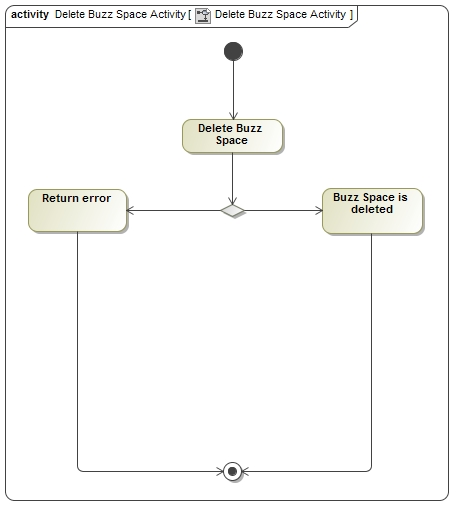
\includegraphics[scale=0.55]{Activity_Diagram__Delete_Buzz_Space_Activity__Delete_Buzz_Space_Activity}
		 \newline
		 
		 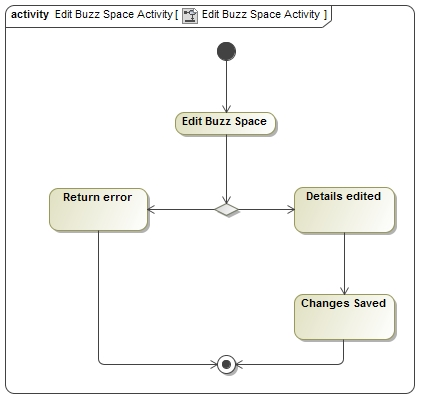
\includegraphics[scale=0.55]{Activity_Diagram__Edit_Buzz_Space_Activity__Edit_Buzz_Space_Activity}
		 \newline
		 
		 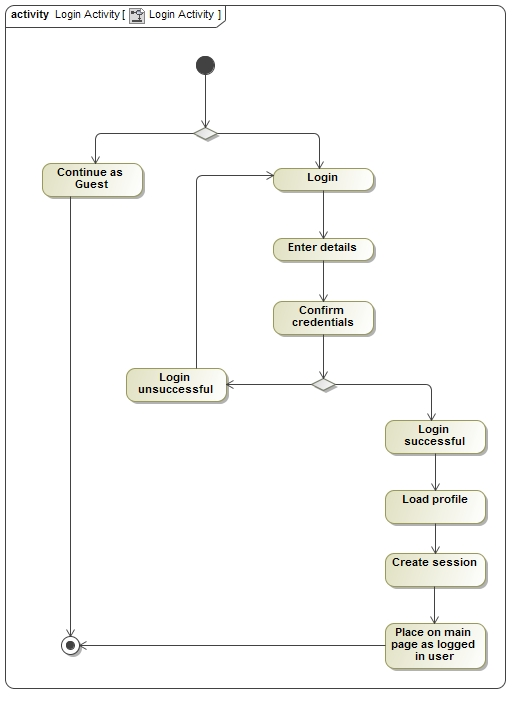
\includegraphics[scale=0.4]{Activity_Diagram__Login_Activity__Login_Activity}
		 \newline
		 
		 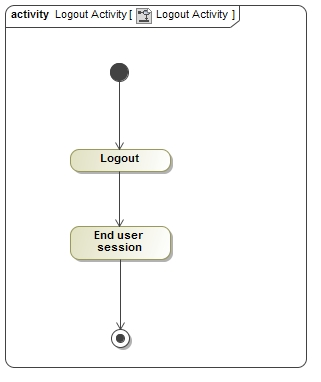
\includegraphics[scale=0.55]{Activity_Diagram__Logout_Activity__Logout_Activity}
		 \newline
		 
		 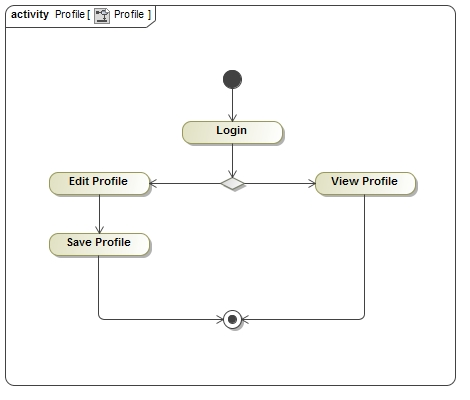
\includegraphics[scale=0.55]{Activity_Diagram__Profile__Profile}
		 \newline
		 
		 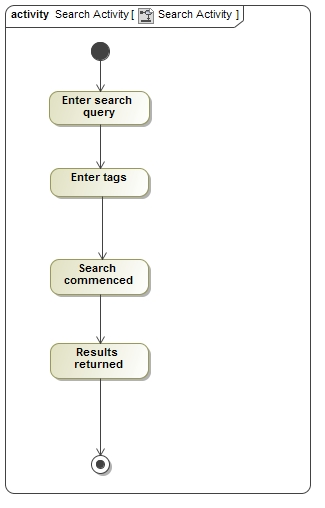
\includegraphics[scale=0.45]{Activity_Diagram__Search_Activity__Search_Activity}
		\newline		 
		 
		 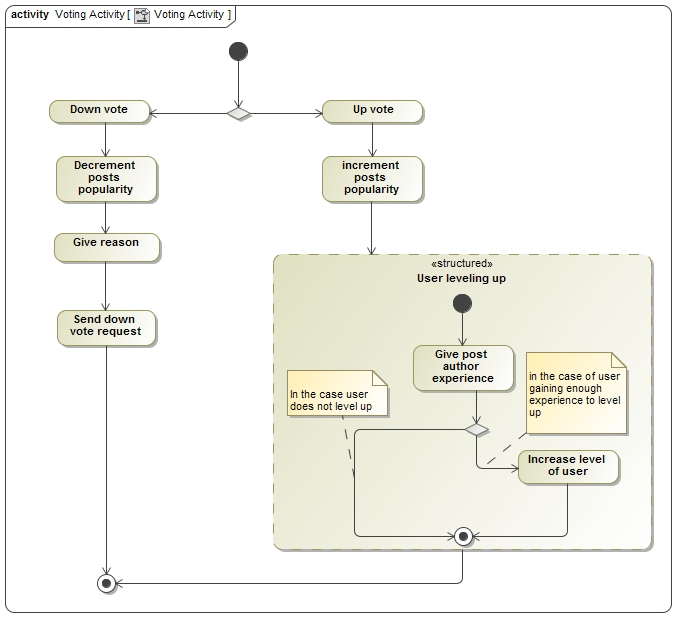
\includegraphics[scale=0.45]{Activity_Diagram__Voting_Activity__Voting_Activity}
		 \newline
		 
 		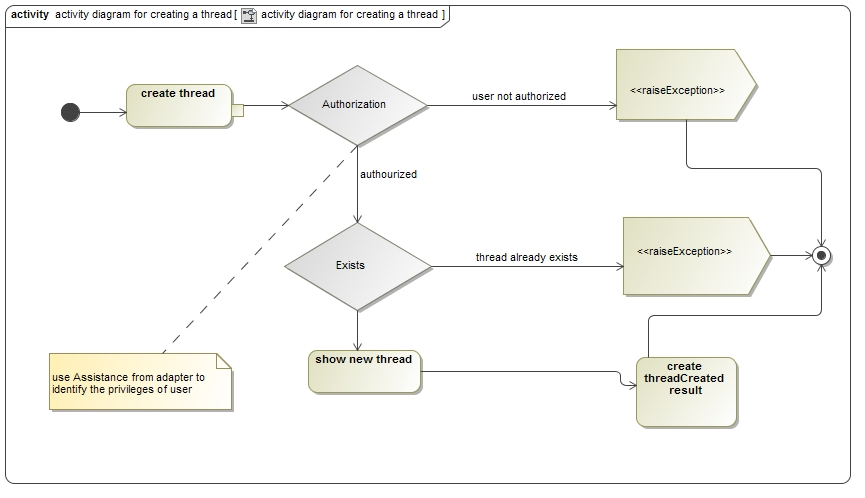
\includegraphics[scale=0.45]{createThreadNew}
		 \newline
		 
		 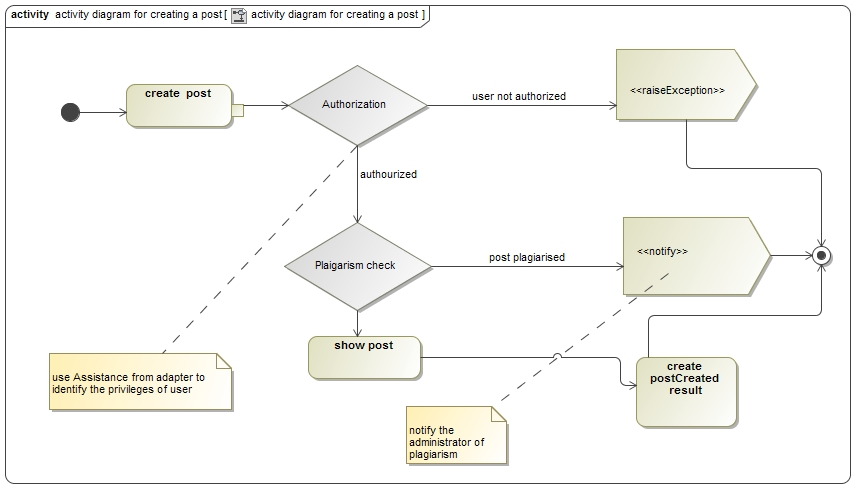
\includegraphics[scale=0.45]{createPostNew}
		 \newline
		 
		  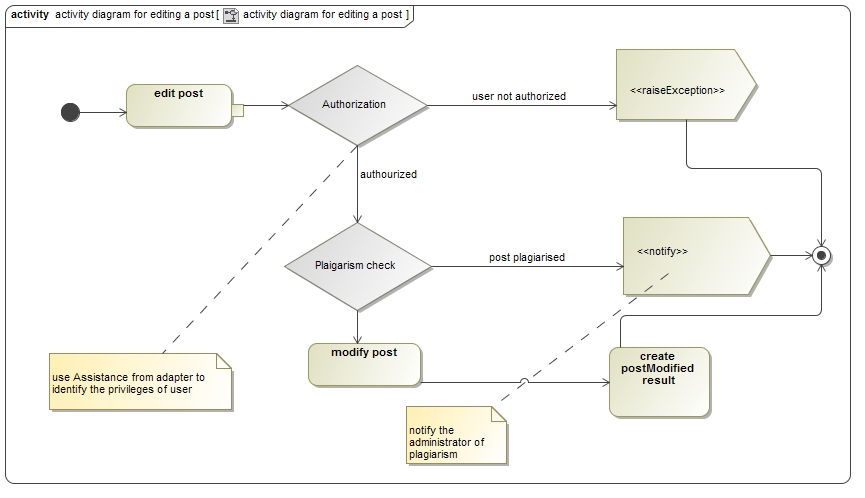
\includegraphics[scale=0.45]{editPostNew}
		 \newline	
		 
		  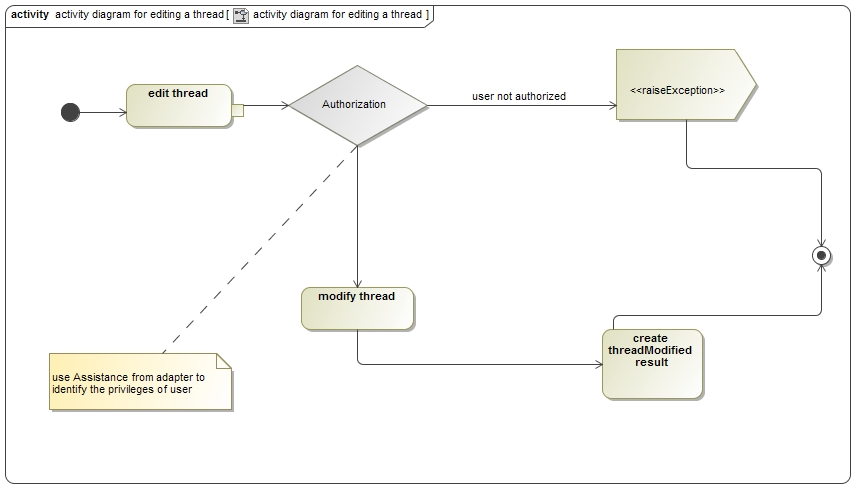
\includegraphics[scale=0.45]{editThreadNew}
		 \newline	 
		 
		  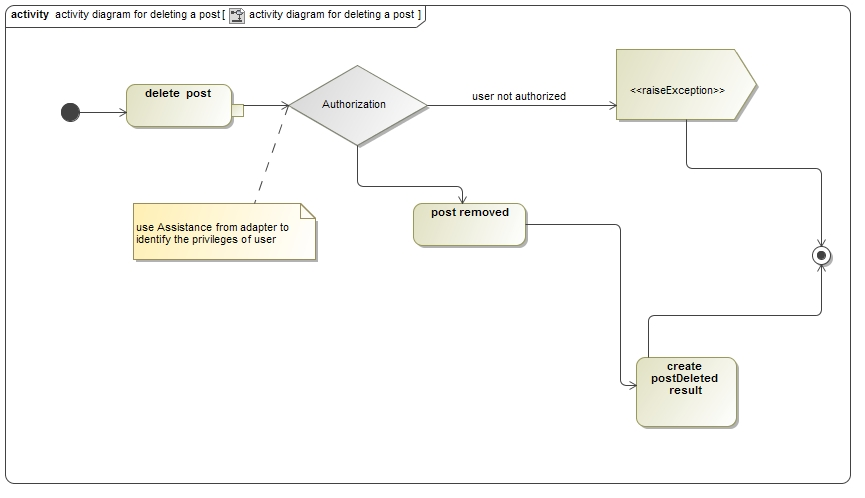
\includegraphics[scale=0.45]{deletePostNew}
		 \newline
		 
		  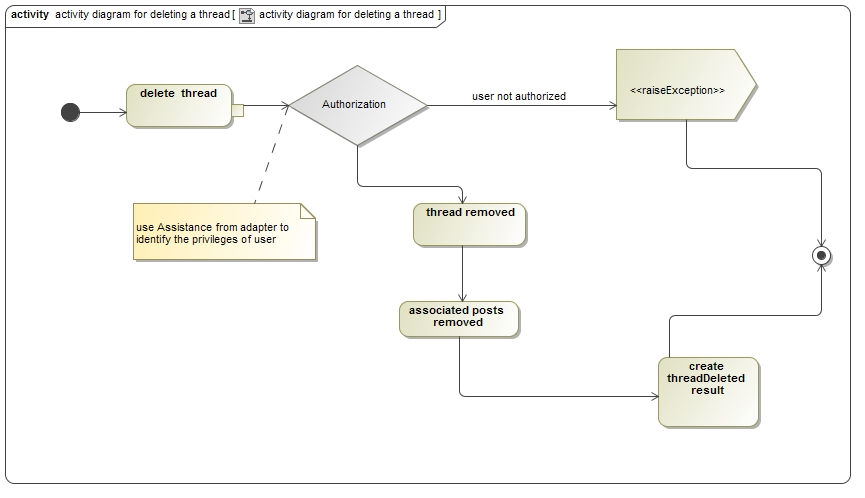
\includegraphics[scale=0.45]{deleteThreadNew}
		 \newline
		 
		  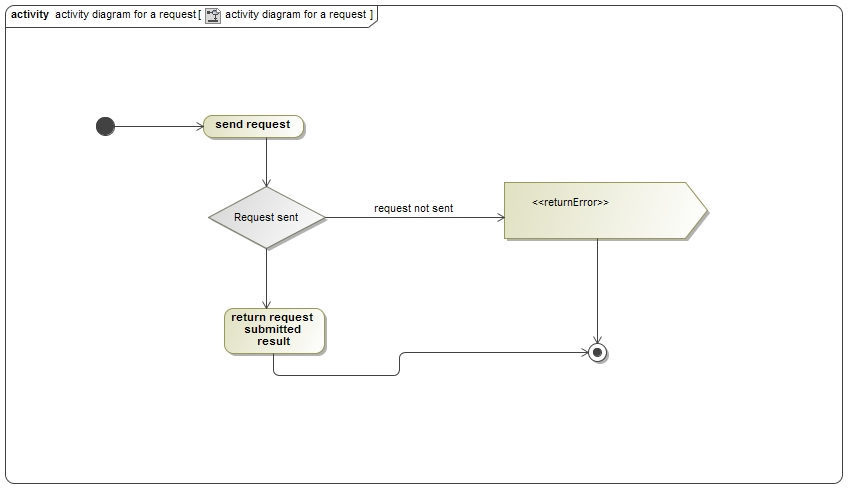
\includegraphics[scale=0.45]{requestNew}
		 \newline
		 
	\subsection{ Domain Model}
		\includegraphics[scale=1]{"Domain Model Diagram"}




\end{document}